\section{Implementing behaviour change theories}\label{sec:bcts}

In this chapter, I design, implement, and parameterise two behaviour change theories (BCTs) within the extended model from the previous chapter. Specifically, I address how integrating theories from psychology into computational models can affect dynamics of disease spread and preventive behaviours. To do so, I adapt and propose methodologies for integrating two distinct BCTs within an agent-based model (ABM), and I investigate the similarities and differences of these implementations. This chapter therefore completes Objectives~\ref{ro3}--\ref{ro5} set out in Section~\ref{sec:research-aims}, laying the foundation for the following chapter which synthesises results from the baseline model, the extended model, and the integration of BCTs.

The structure of this chapter is as follows: First, I explain the importance of psychological BCTs in the context of vector-borne disease (VBD) spread and discuss prior attempts to integrate BCTs within ABMs. Then, I detail my computational implementations of the two BCTs in the extended model. Finally, I assess the impacts of integrating BCTs through two hypothetical scenarios and sensitivity analysis, and I conclude by discussing the implications of my findings within epidemiological and computational modelling contexts.

\subsection{Psychological behaviour change theories}

Psychological BCTs propose mechanisms for why individuals change their behaviour, and as a result, can explain the preventive behaviours of populations. As outlined in greater detail in Section~\ref{sec:lit-review-bcts}, BCTs draw on socio-psychological phenomena to define \textit{constructs}---contextual and personal factors of individuals that combine to explain individual behaviours. In VBD contexts, self-protection is typically a voluntary action involving the use of preventive measures, such as sleeping under insecticide-treated bed nets (ITNs) or applying mosquito repellent. Therefore, understanding the individual factors that drive preventive behaviours within at-risk populations is crucial not only for forecasting disease spread, but also for designing effective health interventions to motivate preventive measure use \cite{vande_velde_integrated_2024}. For these reasons, integrating theories of behaviour change into computational models of disease spread presents an opportunity to explore how preventive behaviours may evolve when grounded in socio-psychological frameworks.

Integrating BCTs into ABMs can create nuanced representations of behaviour and enrich models with emergent, evolving patterns of preventive behaviours. Previous studies have formalised and incorporated BCTs into ABMs to examine how dynamic agent decision-making influences disease spread \cite{durham_incorporating_2012, abdulkareem_risk_2020, weston_infection_2018, bedson_review_2021}. Successful efforts, such as those by \citet{durham_incorporating_2012} and \citet{kurchyna_seeing_2024}, have demonstrated the utility of integrating BCTs for providing mechanistic explanations of preventive behaviour dynamics. Because BCTs are formulated from the perspective of individuals, they are inherently aligned with the agent-based approach. The main challenge, however, lies in translating these theoretical frameworks into computational ones \cite{durham_incorporating_2012}. Despite this, prior research provides a strong foundation for adapting and integrating the two BCTs examined in this thesis into the extended model of VBD spread presented in Chapter~\ref{sec:extended_model}.

\begin{figure}[htbp]
     \centering
     \vspace{.5cm}
     \begin{subfigure}[b]{\textwidth}
         \centering
         \begin{adjustbox}{center}
              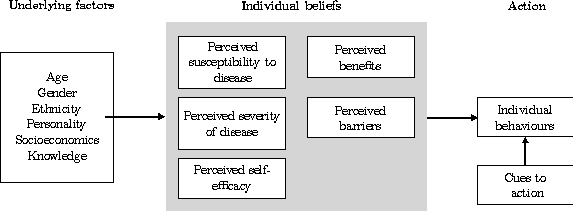
\includegraphics[width=1\textwidth]{figures/ch5/hbm-conceptual-diagram.pdf}
         \end{adjustbox}
         \caption{\textbf{Health Belief Model}}
         \label{fig:hbm-conceptual-comparison}
     \end{subfigure}%
     \\ \vspace{1cm}
     \begin{subfigure}[b]{\textwidth}
         \centering
         \begin{adjustbox}{center}
            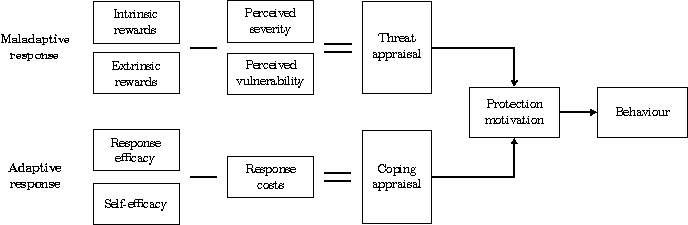
\includegraphics[width=1.2\textwidth]{figures/ch5/pmt-conceptual-diagram.pdf}
         \end{adjustbox}
         \caption{\textbf{Protection Motivation Theory}}
         \label{fig:pmt-conceptual-comparison}
     \end{subfigure}
    \bcaption{Conceptual formulations of chosen behaviour change theories.}{\textbf{(i)} HBM, adapted from \citet{champion_health_2015}. \textbf{(ii)} PMT, adapted from \citet{norman_protection_2015}. Re-displayed here from Figures~\ref{fig:lit-review-hbm} and \ref{fig:lit-review-pmt} for convenience.}
    \label{fig:bct-conceptual-comparison}
\end{figure}

I adapt the extended model to include computational formulations of the Health Belief Model (HBM) and Protection Motivation Theory (PMT). These two BCTs are particularly suited for this research for the following reasons: First, while many BCTs can be applied to protective health behaviours \cite{vande_velde_integrated_2024}, both the HBM and PMT have frequently been used in studies relating to VBD spread (e.g., \cite{watanabe_determinants_2014, yirsaw_insecticide-treated_2021, donohoe_tick-borne_2018} for the HBM; \cite{ghahremani_effect_2014} for PMT). Second, as shown in Figure~\ref{fig:bct-conceptual-comparison}, both BCTs share relatively simple and comparable structures, with overlapping constructs related to the perceived severity and susceptibility to a disease, and the perceived benefits of---and barriers to---adopting a preventive measure \cite{marikyan_protection_2023, weinstein_testing_1993, champion_health_2015}. Lastly, mathematical formulations for both theories already exist, and have been specifically designed for integration within ABMs \cite{durham_incorporating_2012,kurchyna_seeing_2024}.

In the next section, I draw on work from \citet{durham_incorporating_2012} and \citet{kurchyna_seeing_2024} to integrate the HBM and PMT into the extended model presented in Chapter~\ref{sec:extended_model}. Instead of assuming fixed proportions of ITN adoption, as in the previous chapter, I use the integrated BCTs to dynamically determine whether agents sleep under ITNs. I then create three experiments to explore how this dynamic decision-making process impacts preventive behaviours and disease spread under each BCT.

\subsection{Methods}

In this section, I describe the integration of the two chosen BCTs---the HBM and PMT---into the extended model. First, I outline the computational formulations of each theory and explain how they are parameterised to the context of ITN use using VBD survey data. Then, I describe the experiments to investigate seasonal VBD risk before comparing the impacts of the two BCTs on the dynamics of preventive behaviours and disease spread.

\subsubsection{Health Belief Model implementation}

\begin{figure}[hbt!]
     \centering
     \begin{adjustbox}{center}
         % 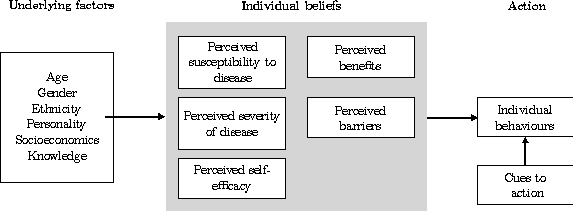
\includegraphics[width=1.2\textwidth]{figures/ch5/hbm-conceptual-diagram.pdf}
         % 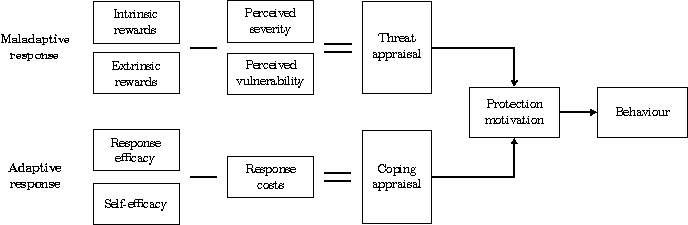
\includegraphics[width=1\textwidth]{figures/ch5/pmt-conceptual-diagram.pdf}
         \resizebox{1\textwidth}{!}{
            %% Creator: Inkscape 1.3.2 (091e20e, 2023-11-25), www.inkscape.org
%% PDF/EPS/PS + LaTeX output extension by Johan Engelen, 2010
%% Accompanies image file 'figures/ch5/hbm-math-diagram.pdf' (pdf, eps, ps)
%%
%% To include the image in your LaTeX document, write
%%   \input{<filename>.pdf_tex}
%%  instead of
%%   \includegraphics{<filename>.pdf}
%% To scale the image, write
%%   \def\svgwidth{<desired width>}
%%   \input{<filename>.pdf_tex}
%%  instead of
%%   \includegraphics[width=<desired width>]{<filename>.pdf}
%%
%% Images with a different path to the parent latex file can
%% be accessed with the `import' package (which may need to be
%% installed) using
%%   \usepackage{import}
%% in the preamble, and then including the image with
%%   \import{<path to file>}{<filename>.pdf_tex}
%% Alternatively, one can specify
%%   \graphicspath{{<path to file>/}}
%% 
%% For more information, please see info/svg-inkscape on CTAN:
%%   http://tug.ctan.org/tex-archive/info/svg-inkscape
%%
\begingroup%
  \makeatletter%
  \providecommand\color[2][]{%
    \errmessage{(Inkscape) Color is used for the text in Inkscape, but the package 'color.sty' is not loaded}%
    \renewcommand\color[2][]{}%
  }%
  \providecommand\transparent[1]{%
    \errmessage{(Inkscape) Transparency is used (non-zero) for the text in Inkscape, but the package 'transparent.sty' is not loaded}%
    \renewcommand\transparent[1]{}%
  }%
  \providecommand\rotatebox[2]{#2}%
  \newcommand*\fsize{8 pt\relax}%
  \newcommand*\lineheight[1]{\fontsize{\fsize}{#1\fsize}\selectfont}%
  \ifx\svgwidth\undefined%
    \setlength{\unitlength}{263.77443695bp}%
    \ifx\svgscale\undefined%
      \relax%
    \else%
      \setlength{\unitlength}{\unitlength * \real{\svgscale}}%
    \fi%
  \else%
    \setlength{\unitlength}{\svgwidth}%
  \fi%
  \global\let\svgwidth\undefined%
  \global\let\svgscale\undefined%
  \makeatother%
  \begin{picture}(1,0.56827175)%
    \lineheight{1}%
    \setlength\tabcolsep{0pt}%
    \put(0,0){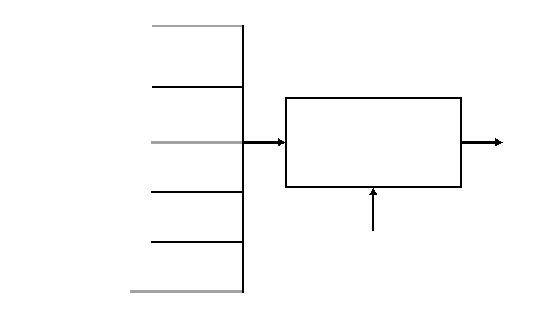
\includegraphics[width=\unitlength,page=1]{figures/ch5/hbm-math-diagram.pdf}}%
    \put(-0.00172156,0.5140235){\color{black}\makebox(0,0)[lt]{\lineheight{1.25}\smash{\begin{tabular}[t]{l}$i=1$\end{tabular}}}}%
    \put(-0.00172156,0.40289279){\color[rgb]{0,0,0}\makebox(0,0)[lt]{\lineheight{1.25}\smash{\begin{tabular}[t]{l}$i=2$\end{tabular}}}}%
    \put(-0.00172156,0.30206003){\color[rgb]{0,0,0}\makebox(0,0)[lt]{\lineheight{1.25}\smash{\begin{tabular}[t]{l}$i=3$\end{tabular}}}}%
    \put(0.5337258,0.30917476){\color[rgb]{0,0,0}\makebox(0,0)[lt]{\lineheight{1.25}\smash{\begin{tabular}[t]{l}$\frac{\text{OR}_0\cdot\text{OR}_2\cdot\text{OR}_4\cdot\text{OR}_5}{1+\text{OR}_0\cdot\text{OR}_2\cdot\text{OR}_4\cdot\text{OR}_5}$\end{tabular}}}}%
    \put(0.33796707,0.5315256){\color{gray}\makebox(0,0)[lt]{\lineheight{1.25}\smash{\begin{tabular}[t]{l}$\text{OR}_1$\end{tabular}}}}%
    \put(0.33796707,0.41880345){\color[rgb]{0,0,0}\makebox(0,0)[lt]{\lineheight{1.25}\smash{\begin{tabular}[t]{l}$\text{OR}_2$\end{tabular}}}}%
    \put(0.33796707,0.22866551){\color[rgb]{0,0,0}\makebox(0,0)[lt]{\lineheight{1.25}\smash{\begin{tabular}[t]{l}$\text{OR}_4$\end{tabular}}}}%
    \put(0.33796707,0.13841411){\color[rgb]{0,0,0}\makebox(0,0)[lt]{\lineheight{1.25}\smash{\begin{tabular}[t]{l}$\text{OR}_5$\end{tabular}}}}%
    \put(0.33796707,0.04634328){\color{gray}\makebox(0,0)[lt]{\lineheight{1.25}\smash{\begin{tabular}[t]{l}$\text{OR}_6$\end{tabular}}}}%
    \put(0.65282162,0.12058035){\color[rgb]{0,0,0}\makebox(0,0)[lt]{\lineheight{1.25}\smash{\begin{tabular}[t]{l}$\text{OR}_0$\end{tabular}}}}%
    \put(-0.00172156,0.21152521){\color[rgb]{0,0,0}\makebox(0,0)[lt]{\lineheight{1.25}\smash{\begin{tabular}[t]{l}$i=4$\end{tabular}}}}%
    \put(-0.00172156,0.12099039){\color[rgb]{0,0,0}\makebox(0,0)[lt]{\lineheight{1.25}\smash{\begin{tabular}[t]{l}$i=5$\end{tabular}}}}%
    \put(0,0){\includegraphics[width=\unitlength,page=2]{figures/ch5/hbm-math-diagram.pdf}}%
    \put(-0.00147328,0.03045556){\color[rgb]{0,0,0}\makebox(0,0)[lt]{\lineheight{1.25}\smash{\begin{tabular}[t]{l}$i=6$\end{tabular}}}}%
    \put(0.33796707,0.31878911){\color{gray}\makebox(0,0)[lt]{\lineheight{1.25}\smash{\begin{tabular}[t]{l}$\text{OR}_3$\end{tabular}}}}%
    \put(0.92511069,0.30484217){\color[rgb]{0,0,0}\makebox(0,0)[lt]{\lineheight{1.25}\smash{\begin{tabular}[t]{l}$p_{\text{ITN}}$\end{tabular}}}}%
  \end{picture}%
\endgroup%

         }
     \end{adjustbox}
         \bcaption{HBM implementation.}{Odds ratios for constructs in a \q{high} state undergo a logistic transformation to calculate the probability of ITN use, $p_{\text{ITN}}$. Constructs in \q{low} states are greyed out (in this case, $i=1,3,6$) and their odds ratios do not contribute to the derivation of $p_{\text{ITN}}$.}
    \label{fig:hbm-implementation}
\end{figure}

I build on work by \citet{durham_incorporating_2012} to integrate the HBM into the extended model using a mathematical representation of the HBM. As shown in Figure~\ref{fig:hbm-implementation}, this formulation calculates the probability of an agent performing the preventive behaviour by combining odds ratios that map to HBM constructs. In my case, the probability that an agent uses an ITN, $p_{\text{ITN}}$, is calculated as:

\begin{equation}\label{eq:prob-hbm}
    p_{\text{ITN}} = \frac{\text{OR}_0\cdot\prod_i{\text{OR}_i^{x_i}}}{1+\text{OR}_0\cdot\prod_i{\text{OR}_i^{x_i}}},
\end{equation}
where each HBM construct is denoted by an index $i\in1,\dots,6$ (or construct names are equivalently used), where $x_i$ is the corresponding indicator variable representing the state of the construct---a \q{high} construct state is defined as $x_i=1$, whereas \q{low} is $x_i=0$. Each term $\text{OR}_{i}$ denotes the odds ratio\footnote{The odds ratio (OR) here is the odds that an agent performs the preventive health behaviour conditional on the construct having a \q{high} state. Equivalently, it is a transformation of the probability the agent adopts the preventive measure. For the $i^{\text{th}}$ construct, $\text{OR}_i=\frac{p({\text{use ITN}}\mid x_i=1)}{1-p({\text{use ITN}}\mid x_i=1)}$.} of an agent performing the preventive behaviour given the $i^{\text{th}}$ construct is in a \q{high} state, or equivalently when $x_i=1$. $\text{OR}_0$ calibrates the value of $p_{\text{ITN}}$ when all HBM constructs are in a \q{low} state. Therefore, this formulation combines the HBM constructs shown in Figure~\ref{fig:hbm-conceptual-comparison} through a transformation of the odds ratios of constructs in \q{high} states to derive a probability of ITN use $p_{\text{ITN}}\in[0,1]$. As the original authors point out, this approach is suited to BCTs since in public health literature (and VBD studies) it is standard convention to \q{describe relationships between belief constructs and behaviour with logistic models} \cite{durham_incorporating_2012}.

I modify this mathematical expression of the HBM to adapt the formulation to the extended model. First, while \citet{durham_incorporating_2012} originally omitted the constructs of self-efficacy and cues to action from their model, I include these in my implementation by adding two more terms to the HBM expression, as shown in Figure~\ref{fig:hbm-implementation}. Second, the original HBM implementation includes a \q{behaviour decision} process in which agents adopt a health behaviour strictly when the probability determined in \eqref{eq:prob-hbm} is at least $0.5$. To better simulate the heterogeneous nature of human decision making, I incorporate random variation in agent decision-making and directly set $p_{\text{ITN}}$ to equal the value in \eqref{eq:prob-hbm}, meaning agents may not use an ITN even if $p_{\text{ITN}}\ge0.5$. Lastly, \citet{durham_incorporating_2012} modelled most values for $x_i$ as dynamic, meaning they were dependent on temporal model and agent attributes. In order to preserve model tractability and low-dimensional realism discussed in Chapter~\ref{sec:extended_model}, I instead hold some constructs fixed---that is, I simply set $x_i=0$ or $x_i=1$ throughout the entire simulation.

Below, for each HBM construct, I first describe how the construct is computationally implemented, and then explain the value chosen for its odds ratio. All parameters for the HBM implementation are provided in Table~\ref{tab:hbm-params}.

\begin{table}[htp!]
    \centering
    \footnotesize
    \begin{adjustbox}{center}
        % \begin{tabular}{p{3cm}p{2cm}p{6cm}p{2cm}p{3cm}} \toprule
        \begin{tabular}{m{3cm} >{\centering\arraybackslash}m{2cm} m{6cm} >{\centering\arraybackslash}m{2cm} m{3cm}} \toprule
        
        Construct & \centering Parameter & Description & \centering Value & Reference \\ \midrule
        & \centering $\text{OR}_0$ & Odds ratio for ITN use when all constructs are in a low state & \centering $1.0$ &  \\ \midrule
        
        Perceived susceptibility ($i=1$) 
        &  & Beliefs regarding risk of becoming infected with disease &  & \citet{champion_health_2015} \\
        & & & & \\
        & \centering $\delta$ & Time discounting rate of disease cases & \centering $0.99$ &  \\
        & \centering $d_c$ & Threshold for high perceived susceptibility & \centering $0.02\times N_h^{(k)}$ & \citet{durham_incorporating_2012} \\
        & \centering $\text{OR}_1$ & Odds ratio for ITN use with high perceived susceptibility & \centering $1.82$ & \citet{mensah_individual_2020} \\ \midrule
        
        Perceived severity ($i=2$) 
        &  & Beliefs regarding the seriousness of disease &  & \citet{champion_health_2015} \\
        & & & & \\
        & \centering $\text{OR}_2$ & Odds ratio for ITN use with high perceived severity & \centering $2.78$ & \citet{kakaire_role_2023} \\ \midrule
        
        Perceived benefits ($i=3$) 
        &  & Beliefs regarding positive outcomes that arise from adopting ITNs &  & \citet{champion_health_2015} \\
        & & & & \\
        & \centering $\text{OR}_3$ & Odds ratio for ITN use with high perceived benefits & \centering $1.47$ & \citet{babalola_factors_2018} \\ \midrule
        
        Perceived barriers ($i=4$) 
        &  & Beliefs about tangible and psychological costs of using ITNs &  & \citet{champion_health_2015} \\
        & & & & \\
        & \centering $\text{OR}_4$ & Odds ratio for ITN use with high perceived barriers & \centering $0.53$ & \citet{yirsaw_insecticide-treated_2021} \\ \midrule
        
        Self-efficacy ($i=5$) 
        &  & Confidence and ability to successfully use ITNs &  & \citet{champion_health_2015} \\
        & & & & \\
        & \centering $itn_{t=0}$ & Initial ITN consistency score & \centering $5$ &  \\
        & \centering $itn_{\max}$ & Maximum ITN consistency score & \centering $10$ &  \\
        & \centering $\text{OR}_5$ & Odds ratio for ITN use with high perceived self-efficacy & \centering $1.3$ & \citet{storey_associations_2018, babalola_factors_2018} \\ \midrule
        
        Cues to action ($i=6$) 
        &  & External stimuli that instigate ITN use &  & \citet{champion_health_2015} \\
        & & & & \\
        & \centering $\omega_c$ & Proportion of ITN adoption in agent's social circle to instigate ITN use & \centering $0.5$ &  \\
        & \centering $\text{OR}_6$ & Odds ratio for ITN use with sufficient cues to action & \centering $2.69$ & \citet{phok_behavioural_2022} \\ \bottomrule
    \end{tabular}
    \end{adjustbox}
    \bcaption{Parameters used in the HBM implementation within the extended model.}{Each row lists the construct, its definition, and any parameters and odds ratios defined with corresponding references.}
    \label{tab:hbm-params}
\end{table}

\paragraph{Perceived susceptibility.}Perceived susceptibility is defined as an individual's beliefs regarding their risk of contracting disease \cite{champion_health_2015}. As \citet{durham_incorporating_2012} point out, the prevalence of disease within an individual's area is often correlated with their perceived risk of infection, and there is a cognitive weighting toward more recent disease cases \cite{funk_modelling_2010}. To capture this phenomenon, \citet{durham_incorporating_2012} determine each agent's perceived susceptibility based on the number of time-discounted cumulative cases of disease in the population $d_t$:

\begin{equation}\label{eq:susceptibility}
    d_t=\sum_{i=0}^{t-2}\delta^i c_{t-i-1},
\end{equation}
which is then compared to a critical threshold value $d_c$ to derive the state of the construct:

\begin{equation*}
    \text{perceived susceptibility}=\begin{cases}
        \text{high} & \text{if } d_t\ge d_c \\
        \text{low} & \text{otherwise.}
    \end{cases}
\end{equation*}

In the above, $c_t$ is the number of new cases at time step $t$, and $\delta\in[0,1]$ is the time discounting rate of cases, where values closer to 1 imply a long cognitive retention of previous cases, whereas values closer to 0 imply attention is only paid to disease cases within the past few days. Similar formulations of susceptibility have appeared in other mathematical infectious disease models \cite{chen_public_2011, poletti_effect_2011}. In the context of VBDs, however, perceived susceptibility of individuals has been shown to be heterogeneous across regions \cite{raude_public_2012}. To adapt this formulation to the extended model, I stratify values for $d_t$ and $d_c$ to create distinct values across the three patches $d_c^{\text{outside}}$, $d_c^{\text{fringe}}$, and $d_c^{\text{inside}}$. By doing so, perceived susceptibility levels differ across the three patches and depend on the new cases within each patch $c_{t}^{\text{outside}}$, $c_{t}^{\text{fringe}}$, and $c_{t}^{\text{inside}}$.

Since the simulation time frame in the extended model is quite short (200 days), I set $\delta=0.99$ to provide agents with a memory of disease cases within preceding days. In \citet{durham_incorporating_2012}, the optimal value for $d_c$ that reproduced the observed real-world disease dynamics was 220 out of 10,000 agents, or roughly 2\% of the population. To proportionally adapt this $d_c$ value across patches, I set $d_c^{(k)}=0.02\times N_h^{(k)}$, where $d_c^{(k)}$ is the threshold for high perceived susceptibility in the $k^{\text{th}}$ patch and $N_h^{(k)}$ is the number of hosts in that patch.

The odds ratio for using ITNs given high perceived susceptibility, $\text{OR}_{\text{susc}}$, varies in the literature. In a survey across Madagascar, Mali, and Nigeria, \citet{storey_associations_2018} found that a higher perceived susceptibility led to a slight \textit{decrease} in observed bed net use, with odds ratios ranging from 0.927--0.998. While this counterintuitive negative correlation between perceived risk of infection and ITN use was also observed by \citet{babalola_factors_2018} ($\text{OR}=0.936$), the authors noted that their results were \q{inconsistent with what some studies have found.} Therefore, I draw on a survey by \citet{mensah_individual_2020} who measured participants' perceived \textit{insusceptibility} to malaria and found a correlation with ITN use. Since the adjusted OR for high perceived insusceptibility was $0.55$, I assume an inverse relationship with susceptibility and take the reciprocal of the OR to derive $\text{OR}_{\text{susc}}=1/0.55\approx1.82$.


\paragraph{Perceived severity.}Perceived severity is the belief about how serious a disease and its consequences are \cite{champion_health_2015}. In \citet{durham_incorporating_2012}, this is encoded by representing how fatal the disease is (or appears to be, through media coverage), where a (reported) high fatality rate leads to high perceived severity. In the extended VBD model, however, the disease is not fatal (agents either recover or remain infected by the end of the simulation), meaning there is no comparable notion of severity. Furthermore, VBD literature suggests little to no temporal variation in individuals' perceived severity to VBDs: While perceived mosquito prevalence and exposure to outdoors are linked to the perceived threat of disease \cite{raude_public_2012}, most VBD studies that measure perceived severity do not elaborate on whether such factors vary over time, and to what degree \cite{kakaire_role_2023, watanabe_determinants_2014, storey_associations_2018, babalola_factors_2018}. For these reasons, perceived severity is fixed in the HBM implementation and does not vary with time---instead, I set the construct to high or low depending on the experiment set-up.% Unlike perceived susceptibility, \textit{severity} concerns not just the likelihood of infection, but also the direct health repercussions that an individual must bear if they become ill. 

Similar to perceived susceptibility, some studies have suggested that high perceived severity is associated with lower rates of bed net use \cite{storey_associations_2018, babalola_factors_2018}. However, the majority of VBD literature suggests perceived severity is positively correlated with protective behaviours \cite{kakaire_role_2023, raude_public_2012, watanabe_determinants_2014, naserrudin_role_2022}. In a study of malaria within Uganda, the odds ratio of ITN use with high levels of perceived threat was $2.78$, so I accordingly set $\text{OR}_{\text{severity}}=2.78$ in the extended model.

\paragraph{Perceived benefits.}The perceived benefits of a health behaviour are an individual's beliefs about the positive outcomes that arise from adopting a preventive measure \cite{champion_health_2015}. In \citet{durham_incorporating_2012}, this was omitted from the HBM implementation in their model because it was unclear how perceived benefits evolved over the course of the epidemic. In VBD contexts, survey data indicate that most individuals perceive ITNs as beneficial tools: One malaria study in north-west Ethiopia found that 53\% of the population perceived ITNs as highly beneficial for malaria prevention \cite{yirsaw_insecticide-treated_2021}. Similarly, 79.4\% of participants in a Vanuatu study believed ITNs prevented malaria \cite{watanabe_determinants_2014}. However, similar to \citet{durham_incorporating_2012}, it is not clear why individuals perceive ITNs as beneficial, or how opinions about the benefits of ITN would evolve over time. Therefore, I fix perceived benefits as high or low in the extended VBD model.

High perceived benefits have been shown to drive ITN adoption in VBD settings \cite{babalola_factors_2018, storey_associations_2018, kakaire_role_2023}. In \citet{kakaire_role_2023}, the adjusted OR of ITN use with a high perceived effectiveness was $1.95$. Similarly, in \citet{babalola_factors_2018}, the adjusted OR was $1.47$. Since the latter study group (caregivers) are more closely aligned to the risk profiles of the extended VBD model than the former study group (pregnant women), I set $\text{OR}_{\text{benefits}}=1.47$.

\paragraph{Perceived barriers.}The perceived barriers of a health behaviour are the tangible (e.g., physical strain or financial hardship) and psychological (e.g., social exclusion or lack of incentives) costs to adopting a preventive measure \cite{champion_health_2015}. In VBD contexts, individuals become averse to ITNs for various reasons, including discomfort due to foul odours, heat, burning or chemical sensations, cleanliness, and misconceptions that ITNs attract bed bugs, are toxic to newborns, are taboo to use, or even cause suffocation \cite{mensah_individual_2020, manuv_investigating_2023, watanabe_determinants_2014, yirsaw_insecticide-treated_2021, naserrudin_role_2022}. In areas with a lack of funding for ITN distribution, cost and availability are also major barriers to adoption \cite{welch_barriers_2012}. However, arguably the most common reason is temperature: In \citet{kakaire_role_2023}, almost a quarter (23.9\%) of participants who reported not sleeping under a bed net claimed it was because the net was \q{too hot.} Likewise in \citet{yirsaw_insecticide-treated_2021}, the most frequent explanation for not sleeping under an ITN was that it was \q{not convenient as it created warm[th].} Since the extended model does not include temperature, this mechanism is implemented by fixing perceived barriers according to the climate of the simulated scenario.

%As listed in the experiments later on in Section~\ref{sec:bct-experiments}, the perceived barriers construct is set to high ($x_{\text{barriers}}=1$) when simulating the hot season, and low ($x_{\text{barriers}}=0$) for the cooler season.
The study from \citet{yirsaw_insecticide-treated_2021} provided an adjusted odds ratio for high perceived barriers of $0.53$. Therefore, in the extended model, I set $\text{OR}_{\text{barriers}}=0.53$.

\paragraph{Self-efficacy.}Self-efficacy is an individual's personal confidence to successfully perform a protective health behaviour \cite{bandura_self-efficacy_1997, champion_health_2015}. This construct was not originally included in the first formulation of the HBM \cite{hochbaum_public_1958}, though when the HBM was later revised by \citet{becker_health_1974}, self-efficacy was included for two reasons: First, to account for individuals' self-assessed levels of competency to perform the health behaviour \cite{bandura_self-efficacy_1997}. Second, to include the expected outcomes of the preventive measure, which are similar---but distinct from---the perceived benefits of the behaviour. While this construct is omitted in \citet{durham_incorporating_2012} due to its recency, I extend the HBM formulation with a term for self-efficacy ($\text{OR}_{\text{self-eff}}$) and I create a mechanism to measure agent self-efficacy levels.

In VBD settings, self-efficacy can play a major role in determining whether individuals exhibit preventive behaviours. As \citet{watanabe_determinants_2014} noted, self-efficacy for ITNs is not only the ability but also the willingness of individuals to properly use ITNs. Because ITN distribution is not an issue in the setting of the extended model (i.e., the Mondulkiri province) \cite{sandfort_forest_2020}, the main factor to determine self-efficacy in the extended model is whether agents possess the sufficient knowledge and confidence to employ ITNs. Consistent ITN use has been found to be positively correlated with self-efficacy \cite{kakaire_role_2023}, and thus in the extended model, I use a similar mechanism to determine self-efficacy. Each agent keeps a record of their ITN use at time step $t$ through the attribute $itn_t$. At each opportunity to sleep under an ITN, agents update their $itn_t$ attributes:

\begin{equation}\label{eq:itn-score}
    itn_{t+1}=\begin{cases}
        \min(itn_t+1,itn_{\max}) & \text{if ITN used} \\
        \max(itn_t-0.25,0) & \text{otherwise.}
    \end{cases}
\end{equation}

That is, agents increase their self-efficacy levels if they sleep under an ITN, and decrease them otherwise. Here, $itn_{\max}$ is the maximum value for $itn_t$ that agents can accrue. The state of the self-efficacy construct is then set:

\begin{equation}\label{eq:hbm-self-efficacy}
    \text{self-efficacy}=\begin{cases}
        \text{high} & \text{if }itn_t\ge\frac{itn_{\max}}{2} \\
        \text{low} & \text{otherwise.}
    \end{cases}
\end{equation}

This mechanism of self-efficacy is formulated such that sleeping under an ITN increases an agent's experience, knowledge, and comfort with ITNs more so than neglecting to sleep under an ITN for one night. The threshold for high self-efficacy depends on $itn_{\max}$, requiring at least $\frac{itn_{\max}}{2}$ days of consistent ITN use in order for the agent to have high self-efficacy. In the extended model, I set $itn_{\max}=10$, meaning agents base their self-efficacy state on the previous $\approx10$--40 days of ITN use, which is aligned with the extensive memory time frame as in perceived susceptibility. I initialise agents with $itn_{t=0}=5$, meaning agents begin with attitudes that border on high self-efficacy.

In \citet{kakaire_role_2023}, the adjusted OR for pregnant women with high levels of self-efficacy was $9.48$, although this was substantially higher compared to other studies. For example, \citet{storey_associations_2018} reported an adjusted OR of $1.34$ in one survey region and $1.20$ in another. Similarly, the adjusted OR for caregivers in \citet{babalola_factors_2018} was $1.238$. Due to these results, I estimate $\text{OR}_{\text{self-eff}}=1.3$ in the extended model.

% \odd{Cues to action}

\paragraph{Cues to action.}Cues to action are prompts or signals that instigate the act of performing a preventive behaviour \cite{champion_health_2015}. Compared to the other constructs in the HBM, cues to action are less well understood, partly because these cues can be anything from physical disease symptoms to subtle mental reminders to exercise self-protective behaviours. Akin to self-efficacy, the cues to action construct is a recent addition to the HBM---although it is mentioned in the original formulation by \citet{hochbaum_public_1958}---and it is similarly excluded from the mathematical HBM formulation by \citet{durham_incorporating_2012}. However, VBD literature suggests cues to action can be a driving force for ITN adoption due to many external stimuli, such as observed media coverage \cite{storey_associations_2018}, messages from health professionals \cite{yirsaw_insecticide-treated_2021}, the distribution of ITNs, and noticeable health campaigns \cite{watanabe_determinants_2014}.

Perhaps the largest external influence on preventive behaviours for individuals in the context of VBDs is the perception of ITNs as a normative social behaviour. This is a common phenomenon for other infectious diseases, where an individual performs a preventive health behaviour not because the individual inherently wants to, but because there is a tacit social pressure or expectation to do so \cite{perkins_agent-based_2019}. Across four VBD-infected regions of Guyana, \citet{lopes-rafegas_contribution_2023} found that risk perception and preventive behaviours were substantially influenced by social norms. Similarly, in their cross-sectional malaria survey in rural Uganda, \citet{perkins_agent-based_2019} found that participants were 2.94 times more likely to sleep under an ITN when they perceived the behaviour as normative in their community. Similar results were observed in \citet{storey_associations_2018, phok_behavioural_2022}.

In the extended HBM formulation, I model ITN use as a social normative behaviour where the amount of social pressure on the $j^{\text{th}}$ agent to sleep under an ITN $\omega_j$ depends on the number of ITNs adopters among the agent's immediate contacts:

\begin{equation}\label{eq:cues-to-action}
    \omega_j=\frac{\text{no. of contacts who used ITNs last night}}{\text{no. of contacts for $j$\textsuperscript{th} agent}},
\end{equation}
where the numerator represents the immediate contacts for the $j^{\text{th}}$ agent who used ITNs the previous night, and the denominator represents the number of immediate contacts for the $j^{\text{th}}$ agent according to the underlying Erdős–Rényi network. If the agent has no contacts, I set $\omega_j=0.5$. The state of the $j^{\text{th}}$ agent's cues to action construct is set as:

\begin{equation}
    \text{cues to action}=\begin{cases}
        \text{high} & \text{if }\omega_j\ge\omega_c \\
        \text{low} & \text{otherwise.}
    \end{cases}
\end{equation}

In the above equation, $\omega_c$ determines the critical threshold for sufficient cues to action to heighten $p_{\text{ITN}}$. This formulation is similar to other infectious disease models that incorporate the diffusion and propagation of preventive behaviours within communities \cite{mao_evaluating_2011, mao_coupling_2012}. In the extended model, I set this threshold to $\omega_c=0.5$ such that the majority of an agent's social circle must adopt ITNs in order for cues to action to be sufficiently present.

The value for $\text{OR}_{\text{cues}}$ chosen to parameterise the construct is from \citet{phok_behavioural_2022}, who studied perceived community social norms toward ITN use for forest-goers, which is aligned with the context of the extended model. I use the adjusted OR determined in the study and set $\text{OR}_{\text{cues}}=2.69$.

\paragraph{$\text{OR}_0$.}I set the calibrating constant $\text{OR}_0=1$, which represents the likelihood of ITN use when all constructs are in a low state. While there are no data available to empirically derive this parameter, this interpretation implies that in the default case, agents adopt ITNs randomly with $p_{\text{ITN}}=0.5$.


\subsubsection{Protection Motivation Theory implementation}

\begin{figure}[hbt!]
     \centering
     \begin{adjustbox}{center}
         \resizebox{1.3\textwidth}{!}{
            %% Creator: Inkscape 1.3.2 (091e20e, 2023-11-25), www.inkscape.org
%% PDF/EPS/PS + LaTeX output extension by Johan Engelen, 2010
%% Accompanies image file 'figures/ch5/pmt-math-diagram.pdf' (pdf, eps, ps)
%%
%% To include the image in your LaTeX document, write
%%   \input{<filename>.pdf_tex}
%%  instead of
%%   \includegraphics{<filename>.pdf}
%% To scale the image, write
%%   \def\svgwidth{<desired width>}
%%   \input{<filename>.pdf_tex}
%%  instead of
%%   \includegraphics[width=<desired width>]{<filename>.pdf}
%%
%% Images with a different path to the parent latex file can
%% be accessed with the `import' package (which may need to be
%% installed) using
%%   \usepackage{import}
%% in the preamble, and then including the image with
%%   \import{<path to file>}{<filename>.pdf_tex}
%% Alternatively, one can specify
%%   \graphicspath{{<path to file>/}}
%% 
%% For more information, please see info/svg-inkscape on CTAN:
%%   http://tug.ctan.org/tex-archive/info/svg-inkscape
%%
\begingroup%
  \makeatletter%
  \providecommand\color[2][]{%
    \errmessage{(Inkscape) Color is used for the text in Inkscape, but the package 'color.sty' is not loaded}%
    \renewcommand\color[2][]{}%
  }%
  \providecommand\transparent[1]{%
    \errmessage{(Inkscape) Transparency is used (non-zero) for the text in Inkscape, but the package 'transparent.sty' is not loaded}%
    \renewcommand\transparent[1]{}%
  }%
  \providecommand\rotatebox[2]{#2}%
  \newcommand*\fsize{8 pt\relax}%
  \newcommand*\lineheight[1]{\fontsize{\fsize}{#1\fsize}\selectfont}%
  \ifx\svgwidth\undefined%
    \setlength{\unitlength}{302.99583435bp}%
    \ifx\svgscale\undefined%
      \relax%
    \else%
      \setlength{\unitlength}{\unitlength * \real{\svgscale}}%
    \fi%
  \else%
    \setlength{\unitlength}{\svgwidth}%
  \fi%
  \global\let\svgwidth\undefined%
  \global\let\svgscale\undefined%
  \makeatother%
  \begin{picture}(1,0.35965502)%
    \lineheight{1}%
    \setlength\tabcolsep{0pt}%
    \put(0,0){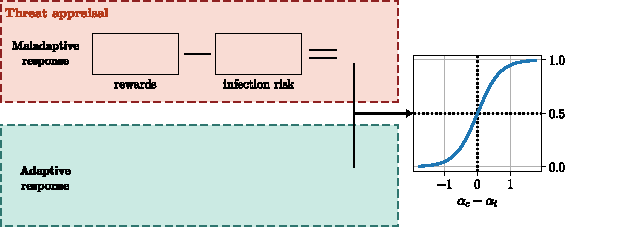
\includegraphics[width=\unitlength,page=1]{figures/ch5/pmt-math-diagram.pdf}}%
    \put(0.17427071,0.26821526){\color[rgb]{0,0,0}\makebox(0,0)[lt]{\lineheight{1.25}\smash{\begin{tabular}[t]{l}$r_i+r_e$\end{tabular}}}}%
    \put(0.36639754,0.26754798){\color[rgb]{0,0,0}\makebox(0,0)[lt]{\lineheight{1.25}\smash{\begin{tabular}[t]{l}$d_s+d_v$\end{tabular}}}}%
    \put(0.54596007,0.27038148){\color[rgb]{0,0,0}\makebox(0,0)[lt]{\lineheight{1.25}\smash{\begin{tabular}[t]{l}$\alpha_t$\end{tabular}}}}%
    \put(0.93480474,0.17493379){\color[rgb]{0,0,0}\makebox(0,0)[lt]{\lineheight{1.25}\smash{\begin{tabular}[t]{l}$p_{\text{ITN}}$\end{tabular}}}}%
    \put(0,0){\includegraphics[width=\unitlength,page=2]{figures/ch5/pmt-math-diagram.pdf}}%
    \put(0.17322204,0.0715618){\color[rgb]{0,0,0}\makebox(0,0)[lt]{\lineheight{1.25}\smash{\begin{tabular}[t]{l}$e_r+e_s$\end{tabular}}}}%
    \put(0.39543995,0.0715618){\color[rgb]{0,0,0}\makebox(0,0)[lt]{\lineheight{1.25}\smash{\begin{tabular}[t]{l}$c_r$\end{tabular}}}}%
    \put(0.54585828,0.07239345){\color[rgb]{0,0,0}\makebox(0,0)[lt]{\lineheight{1.25}\smash{\begin{tabular}[t]{l}$\alpha_c$\end{tabular}}}}%
    \put(0,0){\includegraphics[width=\unitlength,page=3]{figures/ch5/pmt-math-diagram.pdf}}%
  \end{picture}%
\endgroup%

         }
     \end{adjustbox}
         \bcaption{PMT implementation.}{Agents assess the threat $\alpha_t$ by weighing the intrinsic and extrinsic rewards $r_i,r_e$ against their perceived severity $d_s$ and vulnerability $d_v$ of disease. The coping appraisal $\alpha_c$ compares the efficacy of the individual $e_s$ and the response $e_r$ against the preventive measure's cost $c_r$. The difference in these appraisals $\alpha_c-\alpha_t$ is transformed via a sigmoid function to derive the probability of protection $p_{\text{ITN}}$. This transformation has the correct directional properties such that higher values of $\alpha_c$ above $\alpha_t$ imply higher probabilities of ITN adoption.}
    \label{fig:pmt-implementation}
\end{figure}

In this section, I outline my implementation of Protection Motivation Theory (PMT) in the extended model. As evident from Figure~\ref{fig:pmt-conceptual-comparison}, PMT shares multiple constructs with the HBM, although the structure of the BCT is different: Unlike the HBM, PMT hypothesises that individuals undergo a cognitive cost-benefit analysis that informs preventive behaviours \cite{rogers_cognitive_1983, norman_protection_2015}. In the terminology of PMT, individuals either exhibit \textit{adaptive} behaviour (in this case, using ITNs) or \textit{maladaptive} behaviour (not using ITNs). To determine the exhibited behaviour, individuals conduct two \textit{appraisals}---the first is the threat appraisal, in which individuals assess what the rewards, risk, and consequences are for maladaptive behaviour. In the coping appraisal, individuals weigh the costs of the adaptive behaviour against its potential health benefits and their confidence and ability to properly use the preventive measure \cite{marikyan_protection_2023}. Below, I first describe how this theoretical framework is computationally implemented in the extended model and I then outline how each PMT construct is represented.

I adapt work from \citet{kurchyna_seeing_2024} to computationally embed PMT as an agent decision-making process. Versions of PMT have previously been implemented in ABMs by \citet{tan_unveiling_2024,ghoreishi_unlocking_2024}. Most notably, \citet{kurchyna_seeing_2024} proposed a formulation of PMT in the context of health behaviours towards smoking. This formulation is general enough to be adapted to other public health contexts, such as for VBDs. Figure~\ref{fig:pmt-implementation} represents the computational implementation of PMT in the extended model. In the representation, PMT constructs ($r_e$, $d_s$, $d_v$, etc.) are numerical inputs over $[0,1]$ that derive the threat appraisal $\alpha_t$ and coping appraisal $\alpha_c$ terms, which ultimately determine whether an agent performs the preventive behaviour.

An agent's threat appraisal is calculated as:

\begin{equation}\label{eq:alpha-t}
    \alpha_t=\frac{1}{2}\left((r_i+r_e)-(d_s+d_v)\right),
\end{equation}
where $r_i$, $r_e$ are the perceived intrinsic and extrinsic rewards for sleeping under an ITN, respectively. $d_s$ is the perceived severity of the VBD, and $d_v$ is the perceived vulnerability of the disease. An agent's coping appraisal is:

\begin{equation}\label{eq:alpha-c}
    \alpha_c=\frac{1}{2}(e_r+e_s)-c_r,
\end{equation}
where $e_r$ is the response efficacy (how effective an agent perceives ITNs to be), $e_s$ is self-efficacy, and $c_r$ is the cost of performing the preventive behaviour. The appraisal terms $\alpha_t,\alpha_c$ are formulated such that $\alpha_t,\alpha_c\in[-1,1]$. In \citet{kurchyna_seeing_2024}, adaptive behaviour was exhibited in agents when $\alpha_c>\alpha_t$ (i.e., when the agent derived more utility from performing the health behaviour than not).

In the PMT formulation used in the extended model, I adapt the original implementation by adding stochasticity to the decision threshold. I apply a sigmoidal transformation as shown in Figure~\ref{fig:pmt-implementation} to the difference between $\alpha_c$ and $\alpha_t$ to capture random variation in agent decision-making:

\begin{equation}
    p_{\text{ITN}}=\sigma\left(\kappa(\alpha_c-\alpha_t)\right)=\frac{1}{1+e^{-\kappa(\alpha_c-\alpha_t)}},
\end{equation}
where $\sigma(\cdot)$ is the sigmoid function and $\kappa$ is a slope parameter controlling the steepness of the logistic curve. This transformation preserves the proportionality between the two appraisals and an agent's likelihood of performing the health behaviour: When $\alpha_c=\alpha_t$ (i.e., the agent has no incentive to use an ITN), $p_{\text{ITN}}=0.5$. When $\alpha_c>\alpha_t$ (i.e., the agent has an incentive to use an ITN), $p_{\text{ITN}}>0.5$, and conversely, when $\alpha_c<\alpha_t$ (the agent has an incentive to \textit{not} use an ITN), $p_{\text{ITN}}<0.5$. I chose $\kappa=3$ as the first whole number such that when $\alpha_c-\alpha_t=1$, $p_{\text{ITN}}>0.95$. This formulation captures random variation in agent behavioural patterns compared to the original deterministic formulation from \citet{kurchyna_seeing_2024}.

In the remainder of this section, I detail each construct of the PMT implementation. Table~\ref{tab:pmt-params} lists all parameters used in the PMT implementation.

\begin{table}[htp!]
    \centering
    \footnotesize
    \begin{adjustbox}{center}
    \begin{tabular}{m{3cm} >{\centering\arraybackslash}m{2cm} m{5cm} m{5cm}} \toprule
        Construct & Parameter & Description & Value/Derivation \\ \midrule
        
        Intrinsic rewards & $r_i$ & Expected inherent benefits for not using ITNs & Fixed (0.5) \\[.5cm]

        Extrinsic rewards & $r_e$ & Expected external benefits for not using ITNs & Dynamic (depends on ITN adoption rate in agent's social circle) \\[.5cm]

        Perceived severity & $d_s$ & Beliefs regarding the seriousness of disease & Fixed (0 or 1) \\[.5cm]

        Perceived vulnerability & $d_v$ & Beliefs regarding risk of becoming infected with disease & Dynamic (depends on prevalence of VBD in patch) \\[.5cm]

        Response efficacy & $e_r$ & Beliefs regarding effectiveness of ITN to reduce disease & Dynamic (depends on ITN adoption rate within an agent's infected contacts) \\[.5cm]

        Self-efficacy & $e_s$ & Confidence in ability to successfully use ITNs & Dynamic (depends on history of ITN use) \\[.5cm]

        Response costs & $c_r$ & Beliefs about tangible and psychological costs of using ITNs & Fixed (0 or 1) \\ \bottomrule
    \end{tabular}
    \end{adjustbox}
    \bcaption{Parameters used in the PMT implementation within the extended model.}{}
    \label{tab:pmt-params}
\end{table}

\paragraph{Intrinsic rewards ($r_i$).}In PMT, intrinsic rewards refer to the expected inherent benefits from maladaptive behaviour \cite{marikyan_protection_2023}---in other words, the utility the agent inherently derives from not sleeping under ITNs. For example, \citet{kurchyna_seeing_2024} included intrinsic rewards as the pleasure an individual experienced from smoking cigarettes. In the context of ITN use, however, there is little evidence of intrinsic non-health benefits for not sleeping under ITNs: Across all ITN surveys, the vast majority of participants were willing to sleep under ITNs \cite{watanabe_determinants_2014, yirsaw_insecticide-treated_2021, manuv_investigating_2023}. Therefore, in the extended model, I set $r_i=0.5$ to create a neutral intrinsic reward in all simulations.

\paragraph{Extrinsic rewards ($r_e$).}In PMT, the extrinsic rewards of a health behaviour are the external benefits an individual derives from not performing the health behaviour \cite{marikyan_protection_2023}. This construct encapsulates social norms: In \citet{kurchyna_seeing_2024}, social pressure to smoke was modelled as an extrinsic reward for agents. Similarly, the perception of ITN use as a normative behaviour can be represented as an extrinsic reward: When ITN use is low in an agent's social circle, there is an extrinsic reward for the agent to copy the majority behaviour and not sleep under an ITN. Conversely, when ITN use is high among an agent's contacts, this reward is diminished. Therefore, the extrinsic reward $r_e$ for an agent is the complement of the cues to action construct $\omega_j$ from the HBM:

\begin{equation}\label{eq:pmt-r-e}
    r_e=1-w_j=1-\frac{\text{no. of contacts who used ITNs last night}}{\text{no. of contacts for $j$\textsuperscript{th} agent}},
\end{equation}
where the subscript $j$ refers to the $j$\textsuperscript{th} agent, as in \eqref{eq:cues-to-action}. Extrinsic rewards are agent-specific, although the notation is omitted for readability. Unlike the HBM, however, there is no threshold value, since construct values in the PMT implementation are continuous rather than indicator variables.

\paragraph{Perceived severity ($d_s$).}The perceived severity construct in PMT is the same as the HBM---how serious agents perceive the risks and consequences of infection to be. For this reason, perceived severity is similarly fixed in the PMT representation as 0 or 1 to maintain consistency across the two BCTs.

\paragraph{Perceived vulnerability ($d_v$).}Perceived vulnerability in PMT is the same construct as perceived susceptibility in the HBM---an individual's beliefs about the likelihood of infection. The PMT implementation therefore uses the same mechanism to derive this construct for agents, but with a continuous formulation instead of a binary representation (as in $x_{\text{susc}}$). First, the time-discounted new disease cases $d_t^{(k)}$ are calculated for an agent's patch $k$ at the current time step $t$. Then, perceived vulnerability is defined as the proportion of the patch threshold value $d_c^{(k)}$ constrained over $[0,1]$:

\begin{equation}
    d_v^{(k)}=\min\left(\frac{d^{(k)}_t}{d^{(k)}_c},1\right)
\end{equation}

\paragraph{Response efficacy ($e_r$).}Response efficacy is the belief that the preventive behaviour will be effective in protecting oneself and others \cite{marikyan_protection_2023}. It is distinct from perceived benefits in the HBM in that response efficacy is concerned solely with the effectiveness of the response (ITNs) rather than all potential positive side effects. To incorporate this construct in the PMT implementation, I modify the extrinsic rewards construct in \eqref{eq:pmt-r-e} to derive an agent's perceived response efficacy:

\begin{equation}\label{eq:response-efficacy}
    e_r=1-\frac{\text{no. of infected contacts who used ITNs last night}}{\text{no. of infected contacts}}.
\end{equation}

By this formulation, agents cognitively associate disease with a lack of ITN use: When an agent's contacts are infected despite using ITNs, the agent perceives ITNs to be low in effectiveness. However, if the infected contacts are not using the preventive measure, the agent estimates response efficacy to be high. This mechanism draws on the phenomenon of individuals to attribute a lack of preventive measure use as a causal explanation for high rates of disease. While this formulation is not meant to resemble realistic human behaviour, it is one hypothesis for how individuals may estimate the effectiveness of a response using observations within their social network.

\paragraph{Self-efficacy ($e_s$).}Self-efficacy is another shared construct with the HBM---it is an individual's confidence in their ability to properly perform the preventive behaviour. Therefore, the construct in the PMT implementation has a similar form as in \eqref{eq:hbm-self-efficacy}. As was the case for perceived vulnerability, however, the PMT construct is continuous and derived as a proportion of $itn_{\max}$:

\begin{equation}
    e_s=\frac{itn_t}{itn_{\max}}.
\end{equation}

\paragraph{Response costs ($c_r$).}The costs of the response (using an ITN) are semantically equivalent to perceived barriers in the HBM implementation. Since perceived barriers are fixed in the HBM, response costs are similarly set to 0 or 1 based on the simulated scenario.


\subsubsection{Experiments}\label{sec:bcts-experiments}

In this section, I present the experiments to assess the impacts of both BCTs on preventive behaviours and disease spread in the extended model. First, I simulate two scenarios representative of the rainy and dry seasons in the Mondulkiri province which are parameterised with qualitative and quantitative survey data. Then, I assess the sensitivity of the integrated BCTs by varying construct values across the scenarios to observe how changes in behavioural attitudes affect ITN use and disease spread.

\paragraph{Seasonal VBD risk.}The climate of the Mondulkiri province is divided into two seasons---the rainy season (June--October) and the dry season (November--May) \cite{pepey_mobility_2022}. In the mosquito abundance survey from \citet{vantaux_anopheles_2021}, the authors found a statistically significant difference in malaria infection risk between the rainy and dry seasons. To assess how seasonal VBD risk influences dynamics of preventive behaviours and disease spread, I simulated 60 model runs in total across two parameter sets that represented the rainy and dry seasons, shown in Table~\ref{tab:bct-experiment-seasons}.

\begin{table}[htp!]
    \centering
    \begin{adjustbox}{center}
    \begin{tabular}{m{4cm} >{\centering\arraybackslash}m{2.5cm} >{\centering\arraybackslash}m{2.5cm} m{8cm}} \toprule
        Parameter & Rainy season & Dry season & Justification/Hypothesis \\ \midrule

        Perceived severity & High & Low & Higher prevalence of mosquitoes in the rainy season increases agents' risk perception \\[.5cm]
        Perceived benefits\textsuperscript{\textdagger} & High & Low & ITNs reduce the nuisance of biting and noise in the rainy season \\[.5cm]
        Perceived barriers (response cost) & Low & High & Higher temperatures in the dry season lead to higher barriers to ITN use \\[.5cm]
        $K_v^{(2)}$& 9,450 & 9,450 & Mosquito densities in the forest region were reported to be similar across seasons \\[.5cm]
        $K_v^{(1)}$ & 8,100 & 3,375 & \multirow{3}{*}{\shortstack[l]{Mosquito densities in the fringe and outside\\forest areas were 2.4x lower in the dry season}} \\[.5cm]
        $K_v^{(0)}$& 2,700 & 1,125 & \\        \bottomrule
        
    \end{tabular}
    \end{adjustbox}
    \bcaption{Experiment set-up for seasonal VBD infection risk.}{Each row denotes a BCT construct and lists its value across seasons with an explanation. $K_v^{(k)}$ parameters are mosquito carrying capacities for the $k$\textsuperscript{th} patch. {}\textsuperscript{\textdagger} indicates HBM-specific parameters.}
    \label{tab:bct-experiment-seasons}
\end{table}

Higher average temperatures in the dry season \cite{rawson_socio-ecology_2009} cause discomfort during ITN use: In \citet{phok_behavioural_2022}, the authors noted that \q{during the dry season, ... [ITN] use often decreased because the weather was hot.} A similar effect was observed in \citet{watanabe_determinants_2014}, where participants \q{slept without ITNs during the dry season when temperatures are very hot and winds quite weak.} Therefore, perceived barriers (or the PMT equivalent, response costs) were set to high in the dry season, and low in the rainy season. Across the 12 mosquito collection sites in \citet{vantaux_anopheles_2021}, mosquito densities during the dry season were $\approx2.4$ times lower compared to the rainy season. However, this was only observed in the fringe and outside forest regions, with the inside forest area retaining the same approximate mosquito density. Therefore, I reduced mosquito densities across the fringe and outside forest patches by this factor for this experiment, but maintained a consistent mosquito density in the inside forest patch.

Higher mosquito density in the dry season was also noticeable by inhabitants of the Mondulkiri province: \citet{phok_behavioural_2022} reported a decrease in ITN use during the dry season with inhabitants citing less mosquitoes as a primary reason. Other studies have also suggested that observable mosquito density can impact perceptions about infection risk \cite{raude_public_2012}. Overall, inhabitants perceive VBDs as less serious issues during the dry season, so I accordingly set perceived severity to low in the dry season, and high in the rainy season. When mosquito density is higher in the rainy season, qualitative survey data suggest inhabitants use ITNs more frequently because of ITNs' ability to reduce the nuisance of mosquito noise and bites \cite{roosa_general_2022}. Therefore, I set agents' perceived benefits of ITNs to high in the rainy season, and low in the dry season.

\paragraph{Varied perceived severity}To assess each BCT's sensitivity to changes in a single construct, I simulated each season with its opposite perceived severity setting: High perceived disease severity in the dry season, and low perceived severity in the rainy season, totalling 30 additional model runs.

\paragraph{Varied initial self-efficacy.}To determine the effects of varying the initial self-efficacy levels within the population, I initialised agents with different self-efficacy values $e_s=\frac{itn_{t=0}}{itn_{\max}}\in\{0\%,50\%,100\%\}$, totalling 45 additional model runs.

\clearpage
\subsection{Results}

Here, I present the results from the experiments in the order they are described above: First, I examine the behaviour of the extended model with integrated BCTs under the simulated rainy and dry seasons. Then, I assess the impacts of varying perceived severity and I investigate how different initial self-efficacy levels can lead to differences in preventive measure adoption and infection dynamics.

\subsubsection{Seasonal infection risk}

\begin{figure}[hbt!]
     \centering
     \adjustbox{width=1\textwidth,center}{%
        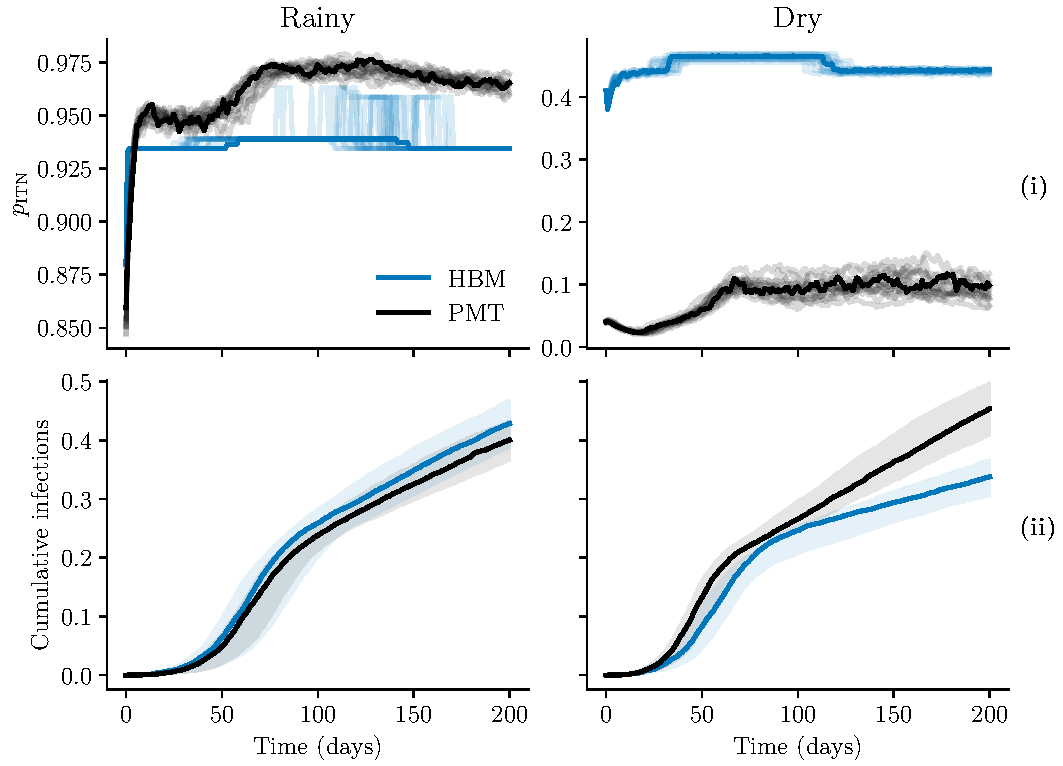
\includegraphics{figures/ch5/1-p-behaviour.pdf}
    }
     \bcaption{Average agent probability of ITN adoption per season and BCT.}{\textbf{(i)} Average probability an agent adopted an ITN per day (note that $y$-axes are different scales). Each line represents one simulation run, and the most representative run (determined using the same methodology as in Section~\ref{sec:extended-model-validation}) is drawn with the highest opacity. \textbf{(ii)} Cumulative infection proportions under both BCTs and seasons. As in Section~\ref{sec:extended-model-results}, shaded bands represent minimum and maximum values across simulation runs. Results for the rainy season were similar in both BCTs, while the PMT implementation led to lower average $p_{\text{ITN}}$ values, and thus higher cumulative infections.}
    \label{fig:ch5-p-behaviour}
\end{figure}

The average probability an agent used an ITN, $p_{\text{ITN}}$, in the rainy scenario was similar in both BCT implementations, as shown in Figure~\ref{fig:ch5-p-behaviour}i. The largest difference was instead observed during the dry season between the HBM and PMT: Agents under the HBM implementation had an average 35--50\% daily chance of adopting ITNs over the course of the simulation, whereas daily values for $p_{\text{ITN}}$ under the PMT implementation were at most 15\%. Supplementary Figure~\ref{fig:ch5-cum-patch} demonstrates how this difference between the BCTs affects infection dynamics across the three patches.

\begin{figure}[hp!]
    \vspace{-1cm}
     \centering
     \adjustbox{width=1.1\textwidth,center}{%
        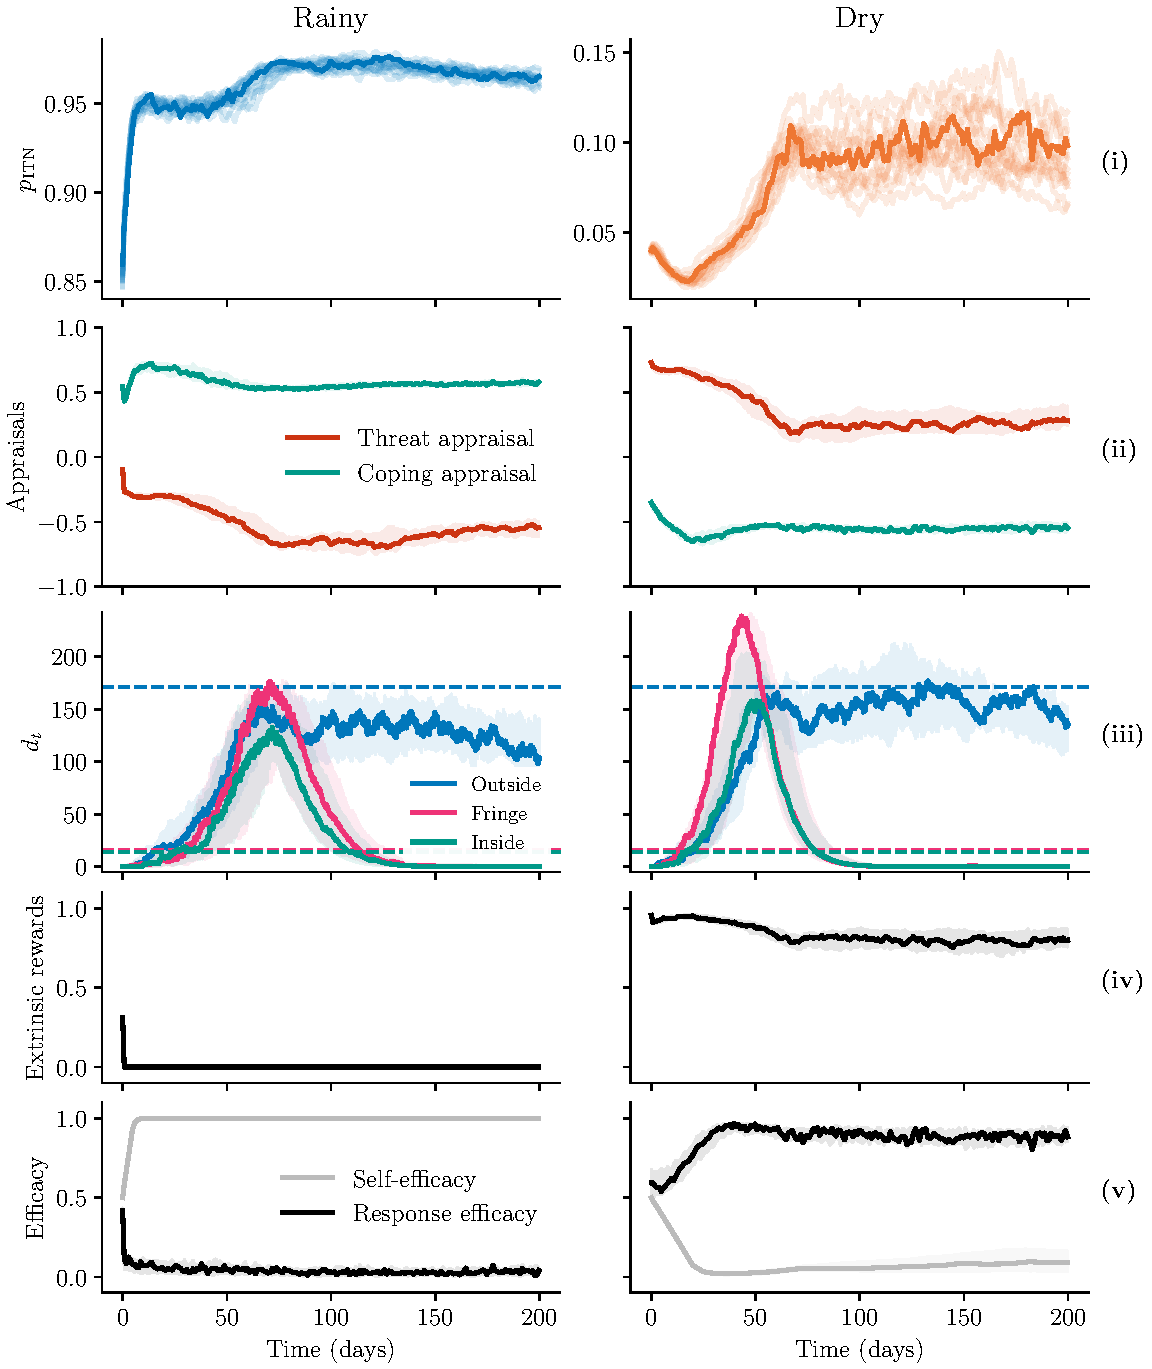
\includegraphics{figures/ch5/5-pmt-determinants.pdf}
    }
     \bcaption{Determinants of ITN adoption probability under the PMT implementation across seasons.}{\textbf{(i)} Average $p_{\text{ITN}}$ values for agents (note that $y$-axes are not shared). \textbf{(ii)} Appraisal values $\alpha_c,\alpha_t$, where higher $\alpha_c$ leads to a higher probability of an agent adopting an ITN. \textbf{(iii)} Time-discounted disease cases per patch $d_t$. Dashed lines represent critical thresholds $d_c$ that saturate an agent's perceived susceptibility. \textbf{(iv)} Average extrinsic rewards $r_e$. \textbf{(v)} Average self-efficacy ($e_s$) and response efficacy ($e_r$) levels.}
    \label{fig:ch5-pmt-determinants}
\end{figure}

Cumulative infections across patches were similar under both BCTs for the rainy scenario, yet varied substantially in the dry season. In the rainy scenario, 95\% infection saturation of the inside and fringe forest patch populations typically occurred by day 85--95 in the HBM and PMT implementations. Interestingly, this period was similar for the HBM during the dry season (80 days on average), but much shorter for PMT (60 days on average). Final cumulative infections for the outside forest patch were also higher under the PMT implementation in the dry season, with an average of 37\% of the population infected compared to 23\% under the HBM.

% \begin{figure}[hbt!]
%      \centering
%      \adjustbox{width=1.2\textwidth,center}{%
%         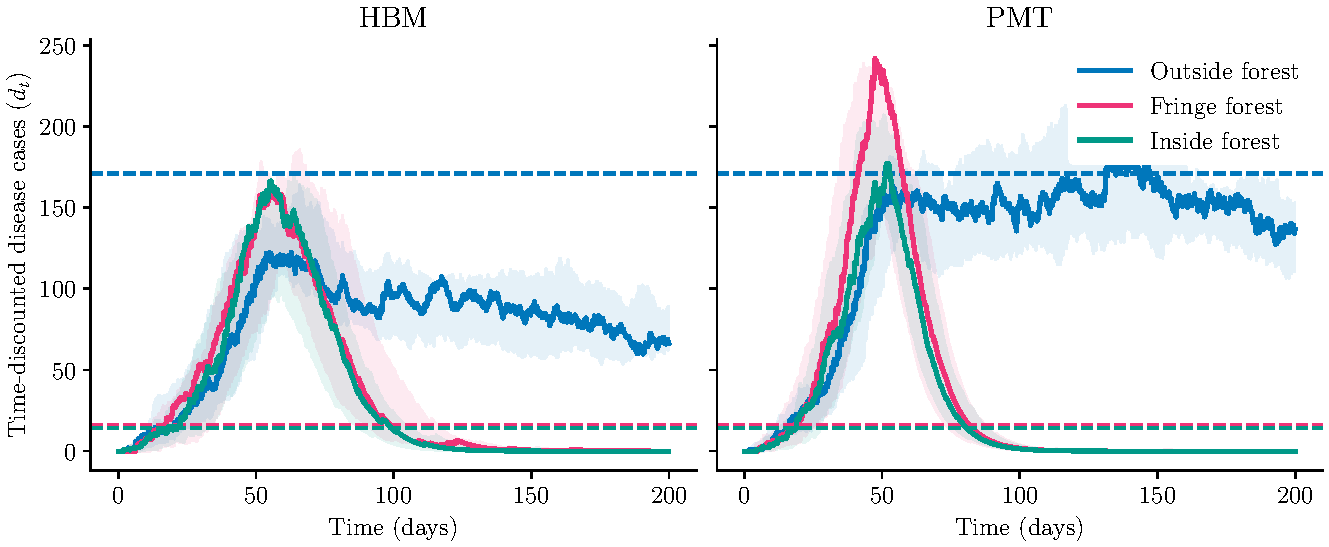
\includegraphics{figures/ch5/3-s-t-dry.pdf}
%     }
%      \bcaption{Disease cases used to derive perceived susceptibility in the dry season.}{Time-discounted new disease cases $d_t$ as defined in \eqref{eq:susceptibility} are shown for each patch. Dashed lines with corresponding colours represent the critical threshold values $d_c$ of each patch that trigger high perceived susceptibility once crossed.}
%     \label{fig:ch5-s-t-dry}
% \end{figure}

% \begin{figure}[hbt!]
%      \centering
%      \adjustbox{width=1.2\textwidth,center}{%
%         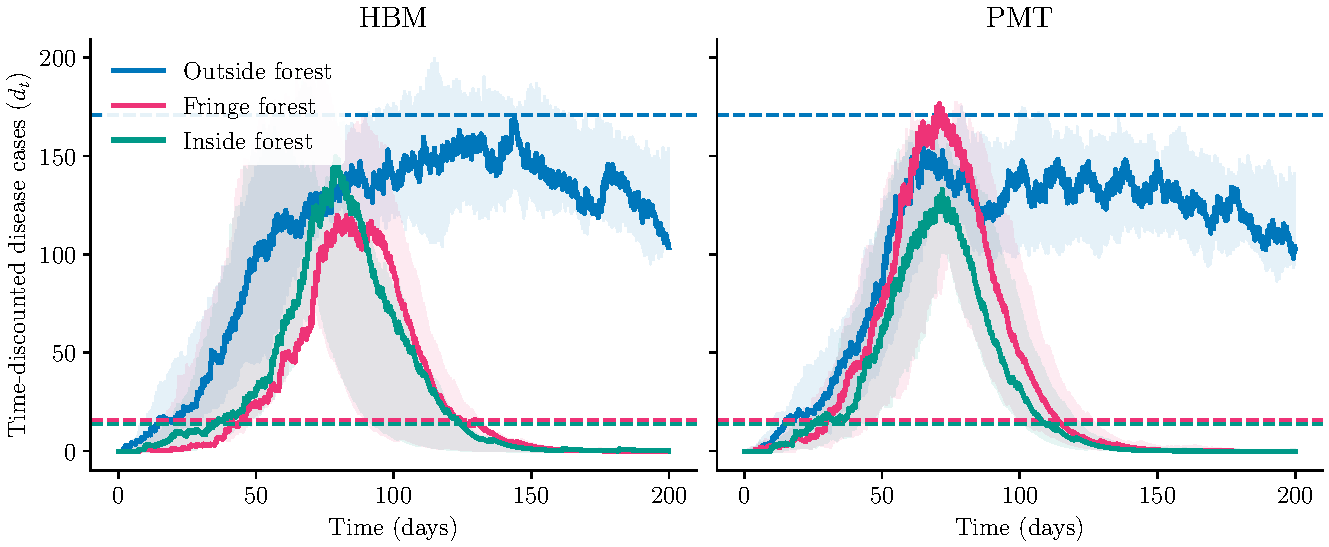
\includegraphics{figures/ch5/4-s-t-rainy.pdf}
%     }
%      \bcaption{Disease cases used to derive perceived susceptibility in the rainy season.}{As in the previous figure, dashed lines represent threshold values for triggering high perceived susceptibility across corresponding colour-coded patches.}
%     \label{fig:ch5-s-t-rainy}
% \end{figure}

Figure~\ref{fig:ch5-pmt-determinants}iii shows the influence of this expedited outbreak under the PMT implementation on agents' perceived susceptibility. Under the PMT implementation, disease cases in the fringe and inside forest patches during the dry season reached higher peaks in less time, and infections in the outside forest patch consistently reached threshold levels for high susceptibility, unlike in the HBM. Contrasted with the rainy season, this phenomenon was somewhat reversed: HBM infections seen in Figure~\ref{fig:ch5-hbm-determinants}ii in the outside forest patch were higher and crossed the high susceptibility threshold more often. That being said, the general downward trend of disease cases across all patches was observed in both BCTs.

\begin{figure}[hp!]
     \centering
     \adjustbox{width=1.1\textwidth,center}{%
        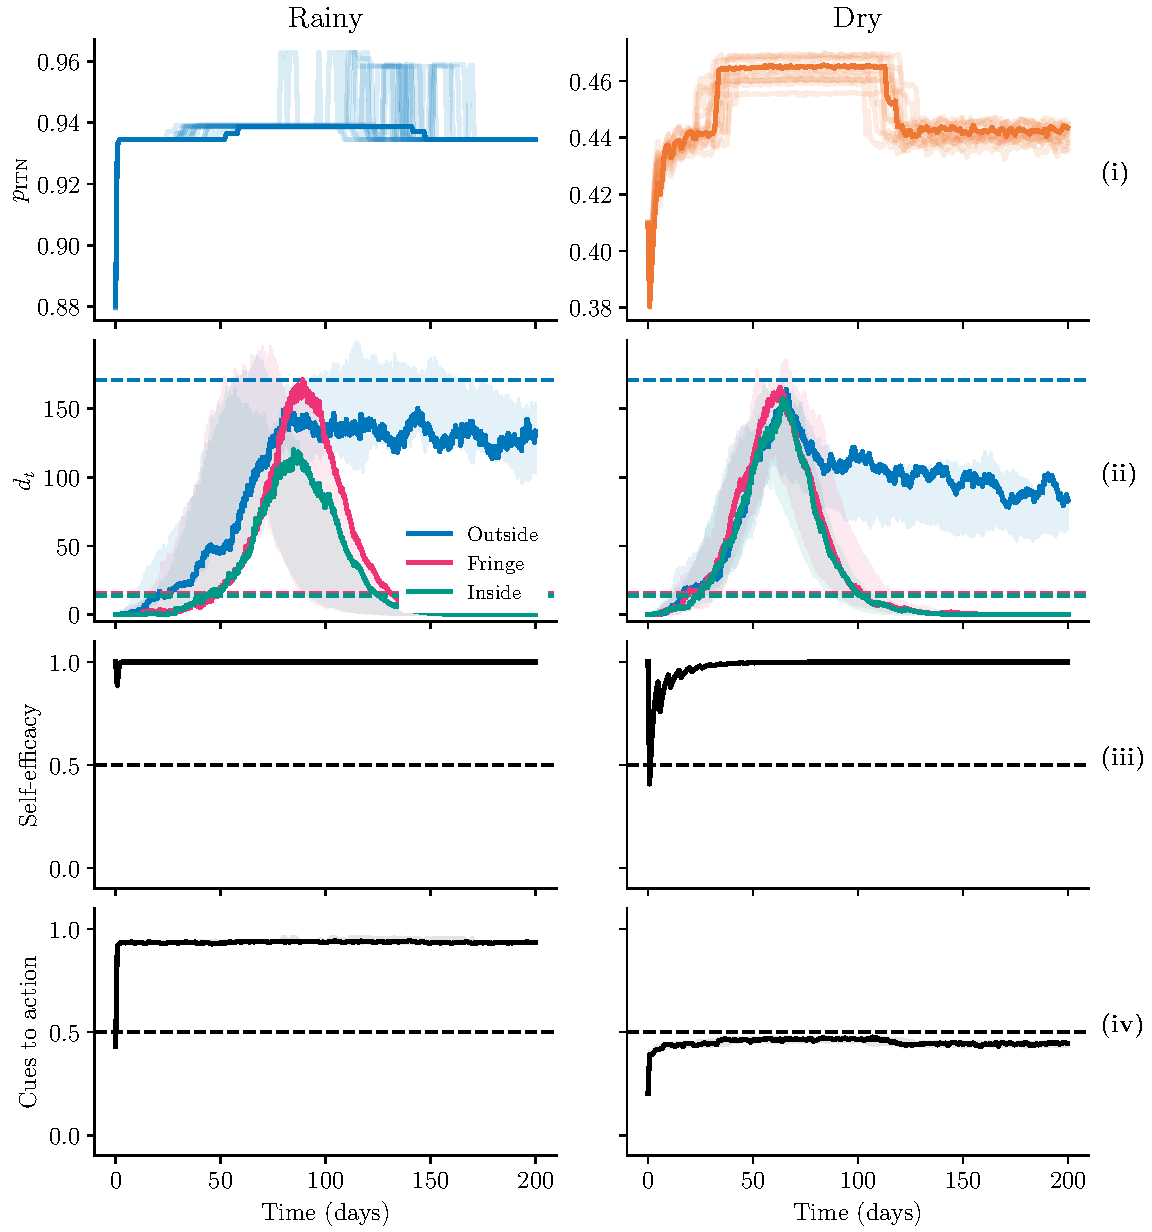
\includegraphics{figures/ch5/6-hbm-determinants.pdf}
    }
     \bcaption{Determinants of ITN adoption probability for the HBM implementation across seasons.}{\textbf{(i)} Average $p_{\text{ITN}}$ values for agents (note that $y$-axes are not shared). \textbf{(ii)} Time-discounted disease cases per patch $d_t$. Dashed lines with corresponding colours represent the critical threshold values $d_c$ of each patch that trigger high perceived susceptibility once crossed. \textbf{(iii)} Average self-efficacy levels. \textbf{(iv)} Average cues to action construct levels. Dashed lines in all plots represent thresholds for high construct states when crossed.}
    \label{fig:ch5-hbm-determinants}
\end{figure}

The influence of perceived susceptibility and other BCT determinants on agents' propensity to use ITNs is conveyed in Figure~\ref{fig:ch5-pmt-determinants} for the PMT implementation. In the rainy season, sleeping under ITNs quickly became a normative behaviour: High perceived severity and low response costs created an initial incentive for agents ($\alpha_c>\alpha_t$) to adopt ITNs, further propelled by the rapid onset of infections in the fringe and inside forest patches, increasing perceived susceptibility. This initial high level of ITN adoption drove an increase in self-efficacy levels, in turn reinforcing the incentive to use ITNs. As self-efficacy increased with adoption, social rewards for rejecting ITNs decreased rapidly.

One surprising result from the rainy season under PMT, however, was low levels of perceived response efficacy. Contrasted with the dry season, response efficacy was high since ITN adoption rates were already low, so the value derived in \eqref{eq:response-efficacy} was naturally close to one. Accordingly, extrinsic rewards to shun ITNs were high since ITN use was not a normative behaviour. This low initial adoption also explains why self-efficacy levels in the dry season were much lower than in the rainy season. The main drivers behind ITN adoption were instead changes in disease cases: Similar to the rainy scenario, infections in the fringe and inside forest patches initially increased ITN adoption. Subsequent variations in ITN adoption were cyclical: Once the temporary push to adopt ITNs wore off, disease cases climbed, and agents were once again incentivised to sleep under ITNs.

Comparing determinants of $p_{\text{ITN}}$ between the PMT and HBM implementations demonstrates the influence of the HBM's threshold formulation. As shown in Figure~\ref{fig:ch5-hbm-determinants}, variations in $p_{\text{ITN}}$ were step-like, initially increasing substantially in the rainy scenario due to a combination of high perceived severity, low perceived barriers, high perceived benefits, and subsequently, sufficient cues to action. Self-efficacy also subsequently rose, similar to the rainy scenario under the PMT implementation. Fluctuating dynamics were observed between preventive measure use and increased disease cases, leading to regular patterns of ITN adoption in the rainy season: When disease cases in the outside forest patch exceeded the critical threshold value, this triggered an increase in $p_{\text{ITN}}$, temporarily increasing ITN adoption, leading to similar cyclical dynamics as in the PMT implementation.

ITN adoption in the dry scenario for the HBM increased rapidly but then decreased and stabilised. Unlike in the rainy scenario, agents' self-efficacy initially dropped, but then increased rapidly alongside disease outbreaks in the fringe and inside forest patches. These two factors drove an increase in average $p_{\text{ITN}}$ to slightly above 46\%. However, once disease cases in the two patches decreased, so did $p_{\text{ITN}}$, to a stable 44\%. The cues to action mechanism was not triggered in the dry season as the probability of ITN adoption across the population was less than the critical threshold of 50\% on average. Additionally, disease cases in the outside forest patch never reached the threshold value for high perceived susceptibility, and infections generally decreased over all simulation runs.

Across the two seasons, there was consistent infection saturation of forest workers due to their high exposure to similar mosquito densities across rainy and dry seasons. Field workers were more likely to be infected in the rainy season compared to the dry season, where higher mosquito densities led to increased infections. This separation was less evident for non-workers, who had comparable final proportions of infections across seasons despite being exposed to 2.4 times less mosquitoes in the dry season. Supplementary Figure~\ref{fig:ch5-hbm-risk-groups} demonstrates these dynamics of disease spread across risk groups in the HBM implementation. 

Disease spread dynamics for the PMT implementation (shown in Supplementary Figure~\ref{fig:ch5-pmt-risk-groups}) were markedly different to those of the HBM implementation. First, forest workers reached saturating infection levels in the dry season before the rainy season, compared to the homogeneous disease spread across seasons under the HBM. Second, cumulative infections for both field and non-workers were higher in the dry season, with the largest difference in non-workers, unlike in the HBM implementation. Lastly, peak epidemic timings occurred sooner in the dry season across all occupations, demonstrating the impact of the lower average $p_{\text{ITN}}$ values compared to the HBM.


\subsubsection{Varied perceptions of disease severity}

\begin{figure}[hbt!]
     \centering
     \adjustbox{width=1\textwidth,center}{%
        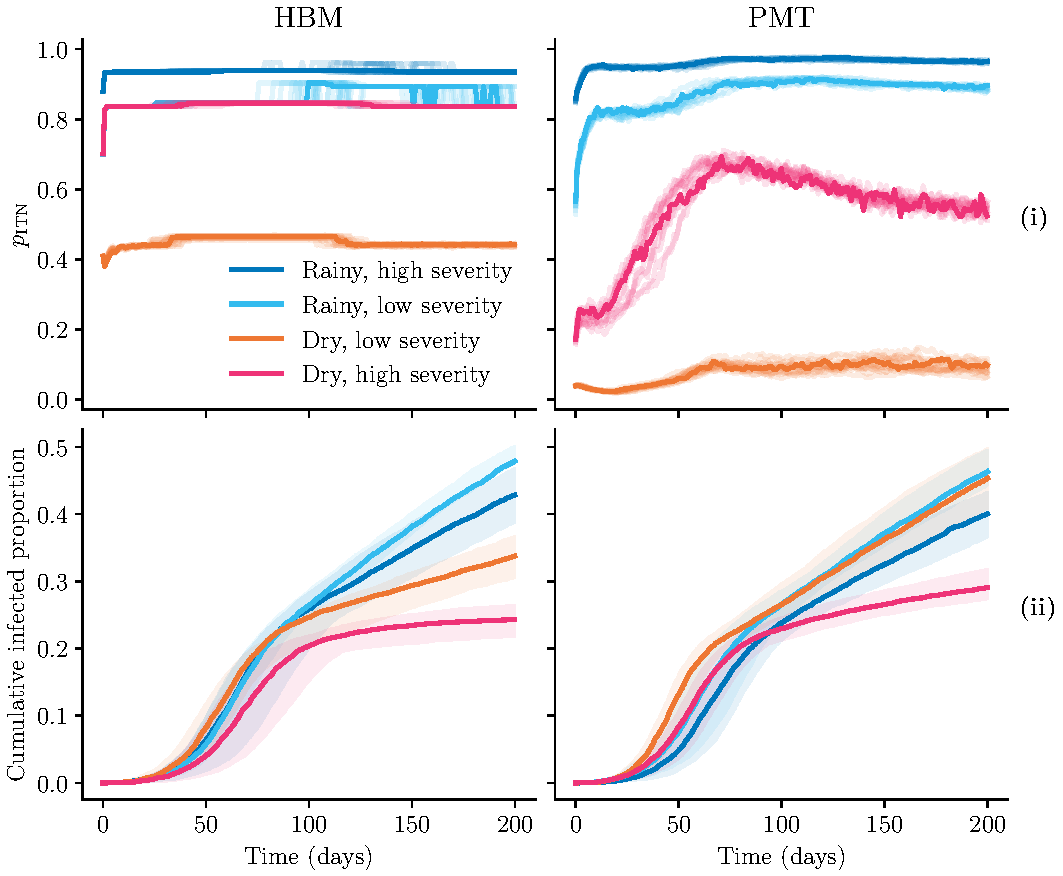
\includegraphics{figures/ch5/ex2-p-beh.pdf}
    }
     \bcaption{Impacts of varying perceived severity on ITN adoption probability across seasons and BCTs.}{\textbf{(i)} Average probability of agents adopting ITNs across BCTs. \textbf{(ii)} Cumulative infection proportions over time. Decreasing perceived severity in the rainy season (light blue) had a marginal impact when compared to increasing perceived severity in the dry season (pink).}
    \label{fig:ex2-p-beh}
\end{figure}

As shown in Figure~\ref{fig:ex2-p-beh}i, decreasing perceived severity in the rainy season had a marginal affect under both BCTs compared to the large increases in $p_{\text{ITN}}$ when perceived severity in the dry season was increased. Under the HBM, increasing agents' perceptions of disease severity during the dry season led to an increased average ITN adoption probability that was just 10\% lower than the average value during the rainy season. Although increasing perceived severity did not lead to $p_{\text{ITN}}$ values as high as the HBM in the PMT implementation, the dynamics of ITN adoption substantially changed: Instead of stagnant adoption as in the low severity scenario, high perceived severity in the dry season led to dramatic increases in ITN adoption, peaking around day 60--70 before gradually declining.

The dramatic increase in average $p_{\text{ITN}}$ values during the dry season with high perceived severity led to the lowest infections across all scenarios. As shown in Figure~\ref{fig:ex2-p-beh}ii, the difference in average total infections between low and high perceived severity for the dry season was higher than in the rainy season under both BCTs. When infections in the dry scenario are examined by occupation (as in Supplementary Figure~\ref{fig:ex2-occupations}) it is clear that increasing perceptions of disease severity lowered the initial and subsequent infections among field and non-workers. This phenomenon was not observed for forest workers, although this is not surprising since infections in forest workers are typically robust to increased ITN adoption rates, as noted in Section~\ref{sec:extended-model-p-itn-impacts}.

\begin{figure}[hbt!]
     \centering
     \adjustbox{width=.8\textwidth,center}{%
        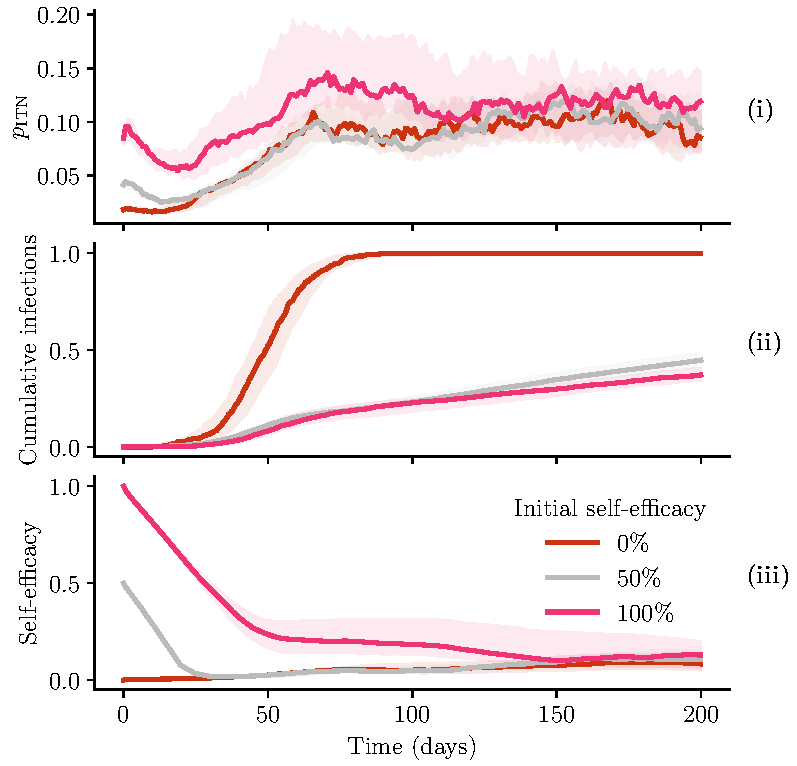
\includegraphics{figures/ch5/ex3-p-itn.pdf}
    }
     \bcaption{Impacts of varying initial self-efficacy levels on ITN adoption and infection dynamics under PMT in dry season with low perceived severity.}{\textbf{(i)} Average probability of agents adopting ITNs. \textbf{(ii)} Cumulative infection proportions on entire population over time. \textbf{(iii)} Average self-efficacy ($e_s$) levels over time. Increasing initial self-efficacy levels from 50\% to 100\% had minimal impact on infection dynamics and ITN adoption. Increasing self-efficacy from 0\% to 50\% did not lead to higher sustained levels of self-efficacy, but prevented a saturating disease outbreak.}
    \label{fig:ex3-p-itn}
\end{figure}

\subsubsection{Increased initial self-efficacy}

When simulated for the dry scenario, increasing initial self-efficacy levels had minimal long-term impacts on agents' probability of adopting ITNs. As shown in Figure~\ref{fig:ex3-p-itn}i and \ref{fig:ex3-p-itn}iii, while higher initial values of self-efficacy led to temporarily increased values for $p_{\text{ITN}}$, self-efficacy levels across all simulations regressed to a similar value of 10\%. Despite this, the impact on disease spread was substantial: Figure~\ref{fig:ex3-p-itn}ii demonstrates how increasing initial self-efficacy levels from 0\% to 50\% prevented a population-wide saturating outbreak of disease by day 75, decreasing infections by an average 85\% at the same point in time across simulations. The impacts of increasing initial self-efficacy levels from 50\% to 100\% were less noteworthy: When agents began with 50\% self-efficacy, 45\% of agents were infected by the end of the simulation compared to 37\% of agents that began with 100\% self-efficacy.

\subsection{Discussion}\label{sec:bcts-discussion}

The results above indicate that integrating BCTs into the extended model of vector-borne disease (VBD) spread from Chapter~\ref{sec:extended_model} altered preventive behaviours of agents, and as a result, influenced dynamics of disease spread. By drawing on mathematical formulations of conceptual theories from psychology, computationally integrating these theories in the extended model allowed for mechanistic explanations of preventive measure adoption. Below, I conclude this chapter by discussing the main similarities and differences between the two implemented BCTs, and discuss the value of my approach and its limitations.

\subsubsection{Similarities and differences of integrated theories}

Despite their differences in formulation, both BCT implementations shared similarities in model output across the experiments. As expected, ITN adoption was heavily reliant on the season in the extended model, with both integrated BCTs exhibiting lower rates of ITN use in the dry season compared to the rainy season. This aligns with trends from the survey data used to parameterise the model \cite{sandfort_forest_2020, vantaux_anopheles_2021}, along with other VBD literature that suggests preventive behaviours are seasonal \cite{phok_behavioural_2022, watanabe_determinants_2014}. Regular oscillations in preventive measure use were observed under both BCTs, both when disease cases were sufficiently prevalent in the rainy season under the HBM, and throughout the PMT implementation. These patterns of cyclical variation in preventive measure adoption alongside disease presence are commonly observed in infectious disease literature \cite{anderson_oscillatory_1984}. 

Increasing agents' perceived disease severity led to increased ITN adoption under both BCTs. This was expected as preventive measure use is typically correlated with perceived disease severity in VBD literature \cite{watanabe_determinants_2014,kakaire_role_2023,raude_public_2012,naserrudin_role_2022}. ITN use as a normative social behaviour was also reflected in both the HBM and PMT implementations: In the HBM, consistent cues to action drove ITN adoption in the rainy season, but adoption was not widespread enough in the dry season to become a social norm. The PMT's unique extrinsic rewards construct meant rewards for not adopting ITNs were lowest during widespread adoption in the rainy season, but high when most agents were not using ITNs. This phrasing of social rewards in PMT as an \textit{alleviating} factor for an agent's threat appraisal, rather than a \textit{driving} force for ITN adoption as in the HBM, highlights a major conceptual difference between the two theories.

One key difference observed between the BCTs was that cumulative infections were higher in the dry season than the rainy season under the PMT implementation, compared to the reverse case in the HBM. Although no data from the Mondulkiri province exist to validate this discrepancy, studies of malaria in similar climates suggest disease transmission during the dry season is greatly reduced \cite{stadler_evidence_2023}, implying the HBM implementation reproduces this trend more faithfully. This increase in infections under the PMT for the dry season compared to the HBM was due to vastly lower average ITN adoption than in the HBM. Re-examining equations \eqref{eq:alpha-t} and \eqref{eq:alpha-c}, this was because fixing perceived severity as low ($d_s=0$) and response costs as high ($c_r=1$) biased the threat appraisal to be consistently larger than the coping appraisal, leading to low initial values for $p_{\text{ITN}}$. In the second experiment, increasing perceived severity in the dry season ($d_s=1$) mitigated this bias, which explains why the PMT implementation exhibited a drastic increase in $p_{\text{ITN}}$ compared to the HBM.

Another difference observed between the two BCTs was self-efficacy during the dry season. While high self-efficacy levels were observed under both BCTs in the rainy season, self-efficacy levels were low in the dry season under PMT when compared to the HBM. This was due to higher average $p_{\text{ITN}}$ values, with almost half of agents adopting ITNs, creating a positive feedback loop for self-efficacy and ITN adoption through the HBM's threshold mechanism. When initial self-efficacy levels were increased under PMT in the final experiment, long-term preventive behaviours were not exhibited, yet disease spread was drastically reduced with the prevention of a saturating outbreak. Not only does this suggest the importance of increasing self-efficacy within at-risk populations, but it also corroborates the idea that health interventions that encourage preventive behaviours should aim to have lasting effects rather than short-term impacts \cite{tapia-conyer_community_2012}.

%Forest workers were impacted the least by changes in perceived disease severity and seasonal variation across both BCTs. As mentioned in Section~\ref{sec:extended-model-validation-results}, this phenomenon is consistent with findings from \citet{sandfort_forest_2020}, who note that while forest workers are a high-risk sub-population, preventing infections in forest workers is challenging due to their constant exposure to VBD-infected areas.

\subsubsection{Strengths and limitations of implementation}\label{sec:bcts-strengths-and-limitations}

The work in this chapter demonstrates how BCTs can be computationally encoded within agents to enrich behavioural decision-making processes and influence dynamics of disease spread. This can allow representations of behaviour that are compartmental, offering insight into the main drivers of preventive behaviours that evolve alongside disease spread. One advantage of this approach in epidemiological contexts is for health officials and policymakers to use such models as test beds for health interventions: Such integrated models of behaviour could be used to determine the most effective behavioural constructs to target with health or communal campaigns as discussed in Section~\ref{sec:lit-review-vec-control} in order to promote preventive behaviours \cite{mateus_c_modeling_2021, linard_multi-agent_2009, scheidegger_agent-based_2017}. For the modelling community, this extended model not only serves as an example of how BCTs can be integrated into ABMs of VBDs, but also demonstrates how different BCTs may considerably influence predictions of disease spread.

However, there are various limitations with integrating BCTs into ABMs that are evident from the work presented here. First, the response efficacy mechanism in the PMT implementation is neither empirically nor qualitatively grounded due to a lack of data available, yet remains a salient factor in determining an agent's behaviour. The low response efficacy exhibited in the rainy season under the PMT implementation suggests that agents are willing to use ITNs but do not believe that ITNs prevent disease, which is contradictory. Because response efficacy is not a construct in the HBM, the HBM implementation does not face the same issue. This highlights how subtle changes in the conceptual formulations of BCTs can impact model dynamics, and also motivates the need for further research into how individuals estimate the efficacy of health interventions.

Another limitation is that the results from the HBM implementation are greatly dependent on defined threshold values. These thresholds determine when agents have \q{high} construct states, triggering large increases in the probability of agents adopting preventive measures. The low adoption of ITNs in the dry season, for example, can be mostly attributed to the threshold value of $\omega_c=0.5$ for the cues to action construct---because average values were slightly below this threshold, a slight decrease in $\omega_c$ would yield higher rates of adoption across the population. This limitation is also acknowledged by \citet{durham_incorporating_2012}, who noted a high dependence on the parameters they used in their HBM implementation. Additionally, holding certain constructs fixed in the PMT formulation from \citet{kurchyna_seeing_2024} can inherently bias the threat and coping appraisals, although this was somewhat mitigated in my implementation by introducing stochasticity. Overall, these drawbacks emphasise the importance of empirically grounded threshold values in the HBM, and well-informed mechanisms of deriving construct values in the PMT implementation.

To conclude, integrating BCTs within the extended model in this chapter demonstrated the possibility of modelling complex dynamics of preventive behaviours and disease spread. However, further work remains necessary to address the drawbacks and limitations of the BCT formulations detailed above. In the next chapter, I discuss avenues for future research in greater detail and aggregate results from Chapters~\ref{sec:baseline_model} and \ref{sec:extended_model}.
